% !TEX encoding = UTF-8 Unicode
% !TEX spellcheck = en_US

\documentclass{svproc}

\usepackage{paralist}
\usepackage{amsmath}
\usepackage{amssymb}
\usepackage{wasysym} % Durchmesser-Symbol
\usepackage{siunitx}
\usepackage{todonotes}
\usepackage{gensymb}
\newcommand{\bm}[1]{\boldsymbol{#1}}
\usepackage[T1]{fontenc} % Für Unterstrich in URL
\usepackage[utf8]{inputenc} % Für Deutsche Umlaute

% Für Bilder
\usepackage{graphicx}
\usepackage{color}
\graphicspath{{./figures/}}

% to typeset URLs, URIs, and DOIs
\usepackage{url}
\def\UrlFont{\rmfamily}

\begin{document}
\mainmatter              % start of a contribution
%
\title{Combined Structural and Dimensional Synthesis of a Parallel Robot for Cryogenic Handling Tasks}
%
\titlerunning{Synthesis of a Cryogenic Handling Robot}
\author{Moritz Schappler\inst{1} \and Philipp Jahn\inst{2} \and Annika Raatz\inst{2} \and Tobias Ortmaier\inst{1}}
%
\authorrunning{Moritz Schappler et al.} % abbreviated author list (for running head)
\institute{Leibniz Universität Hannover, $^1$
Institut für Mechatronische Systeme, An der Universität 1, 30823 Garbsen, Germany,
\email{moritz.schappler@imes.uni-hannover.de},\\ $^2$
Institut für Montagetechnik, An der Universität 2, 30823 Garbsen, Germany}

\maketitle              % typeset the title of the contribution

\begin{abstract}
The combined structural and dimensional synthesis is a tool for finding the robot structure that is suited best for a given task by means of global optimization.
The handling task in cryogenic environments gives strong constraints on the robot synthesis, which are translated by an engineering design step into the combined synthesis algorithm.
This allows to reduce the effort of the combined synthesis, which provides concepts for alternative robot designs and indications on how to modify the existing design prototype, a linear Delta robot with flexure hinges. Promising design candidates are the 3\underline{P}RRU and 3\underline{P}RUR, which outperform the linear Delta (3\underline{P}UU) regarding necessary actuator force.
\keywords{Combined structural and dimensional synthesis, cryogenic work environment, flexure hinge, joint range constraint, parallel robot}
\end{abstract}
%
\section{Introduction and State of the Art}
%

The automation of handling processes is an omnipresent factor in industry and research institutions. 
A robot-supported automation solution is also desirable for extremely niche areas such as the cryogenic storage of biological materials \cite{BorchertLoeBruCar2013}.
The development of task-adapted structures for such exceptional cases poses significant challenges for designers: From an almost infinite variety of design possibilities, the optimal design for the task and the underlying geometric and situational constraints must be found. 
Even if the application's basic parameters are entirely known, it is impossible to manually design and evaluate all possible variations of the robot structure.
One approach to realize all these variations is the computer-aided structural analysis using optimization algorithms. 
In this paper's context, such an optimization strategy is investigated using the example of a parallel robot for use in a cryogenic working environment, and the results are compared with the structure aimed at so far.

It is well established that the performance of parallel robots is highly subject to their kinematic parameters which can be determined for a given structure in a \emph{dimensional synthesis} \cite{Merlet2006}.
The selection of the specific structure, i.e. the \emph{structural synthesis}, is usually performed manually with the help of design and construction principles \cite{FrindtKreHes2010}.
As the systematic structural synthesis of parallel robots by means of screw theory \cite{KongGos2007} or evolutionary morphology \cite{Gogu2008} provides a high number of suitable structures, the selection of the optimal solution is an exhaustive task.
The concept of \emph{combined structural and dimensional synthesis}, introduced in \cite{Krefft2006} for parallel robots, assumes that the optimal solution can be found by independently optimizing all possible structures and selecting the best one.
This requires a high number of simulations of the robots kinematics and dynamics and is only applicable with a general, yet efficient model and its implementation and a suitable optimization algorithm.

The engineering solution to the considered handling problem is the linear Delta robot.
It was already subject to parameter optimizations regarding workspace-related objectives \cite{StockMil2003} or objectives related to kinematics and dynamics \cite{KelaiaiaComZaa2012}.
A dimensional synthesis for both the classical Delta robot and the linear Delta was performed in \cite{Krefft2006} and used for a systematic comparison of the two.

The comparison of multiple parallel robots (whether two different structures or two sets of parameters for one structure) has to be performed using multiple criteria \cite{Merlet2006}, representing all requirements to the robot.
Often genetic algorithms are employed such as the Strength Pareto Evolutionary Algorithm \cite{KelaiaiaComZaa2012,Krefft2006} or Nondominated Sorting Genetic Algorithm \cite{JamwalHusXie2015}.
Particle swarm optimization (PSO) is reported to have better convergence than genetic algorithms for constraint nonlinear optimization problems.
One reason is that not only the parameters of the current iteration carry information but also past iterations are taken into account to generate a new set of parameters \cite{CoelloPulLec2004}. 
Constraint handling \cite{Mezura-MontesCoe2011} is central for the validity of the robot synthesis and the convergence of the PSO.

This paper presents results for the combination of the engineering solution and the combined synthesis presented above by taking the most restricting constraints of the task into account for the structural synthesis and thereby vastly reducing the amount of possible structures, for which a dimensional synthesis has to be performed.
The contributions of the paper are
\begin{compactitem}
\item transferring the specific constraints of cryogenic handling tasks in a suitable form for parameter optimization,
\item proving the applicability of multi-objective PSO on the dimensional synthesis of parallel robots as opposed to genetic algorithms in literature,
\item presenting design alternatives of the linear Delta for cryogenic handling.
\end{compactitem}

The remainder of the paper is structured as follows: 
Sec.\,\ref{sec:taskdef_requ} gives an overview of the constraints of the cryogenic handling task.
The engineering approach to the robot synthesis is presented in Sec.\,\ref{sec:engineering_synthesis}, followed by the combined synthesis in Sec.\,\ref{sec:combined_synthesis}.
The results are discussed in Sec.\,\ref{sec:results}.

%%%%%%%%%%%%%%%%%%%%%%%%%%%%%%%%%%%%%%%%%%%%%%%%%%%%%%%%%%%%%%%%%%%%%%%%%%%%%%%%%%%%%%%%%%%%%%%%%%%%%%%%%%%%%%%%%%%%%%%%%%%%%%%%%%%%%%%%%%%%%%%%%%
\section{Task Definition and Requirements}
\label{sec:taskdef_requ}

The freezing and storage of biological material in biobanks at temperatures below \SI{-130}{\celsius} is commonly referred to as cryopreservation. 
Manual handling of biological or toxic samples is still the norm in research institutions. 
In such systems, the samples are often transferred in, out, or moved by hand using bulky protective clothing. 
This poses considerable risk of injury to the worker through cold burns as well as a threat to the sample integrity. 
% Neuer Absatz wegen Seitenumbruch:

To overcome these problems, a parallel robot for the realization of full automation is being developed.

\subsection{Requirements for the Parallel Robot}
\label{sec:req_robot}

The possibility of placing the drives in the warm area outside the storage container makes the parallel structure interesting for use in cryogenic environments, as it allows the drive technology to be decoupled from the cryogenic handling area. 
The drive movement is then transferred to the end effector platform via passive joints.

The robot to be developed is subject to a number of geometric constraints.
The installation space dimensions correspond to the internal dimensions of the Cryotherm \textsc{Biosafe} cryogenic storage container, which is to be used for the demonstrator (Fig.~\ref{fig:Tank}, left). 
The usable interior space (height \SI{680}{\milli\metre}  and inner diameter \SI{600}{\milli\metre}) is highlighted by the red dashed line in the middle of Fig.~\ref{fig:Tank}. 

\begin{figure}[b!]
    \centering
    \vspace{-0.5cm} % exploit whitespace
	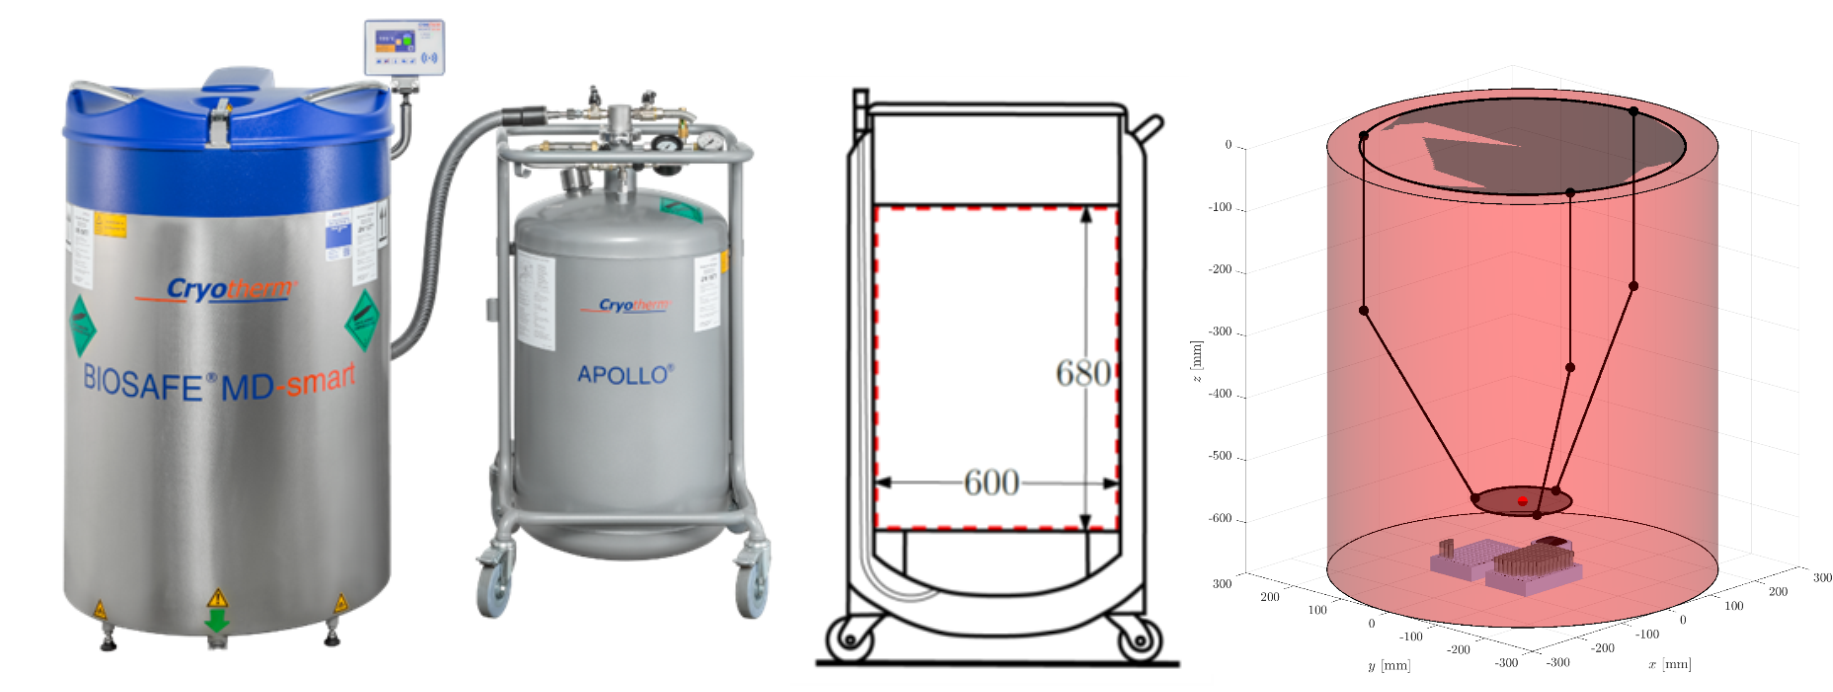
\includegraphics[width=\textwidth,height=\textheight,keepaspectratio]{figures/Tank.png}
	\vspace{-0.7cm} % exploit whitespace
	\caption{Left: Cryotherm \textsc{Biosafe} cryogenic storage container, middle: dimensions of the installation space, right: robot handling scenario in a \textsc{Matlab} simulation.}
	\vspace{-0.5cm} % bring next chapter on this page
	\label{fig:Tank}
\end{figure}

For the storage of sample tubes in the cryogenic storage container, racks of type Micronic 96-3 are to be used, between which the tubes are to be transferred by the manipulator (see Fig.~\ref{fig:Tank}, right). 
The rack's height, including the sample tubes, is \SI{45.2}{\milli\metre}, and the sample tubes height is \SI{44}{\milli\metre}. 
To avoid collisions between the sample tubes to be transferred and the sample tubes stored in the racks during the pick-and-place process, the height of the necessary working space is set to \SI{110}{\milli\metre}, to ensure a safety distance of approx. \SI{20}{\milli\metre}. 
To keep the working space area as small as possible, the racks are placed lengthwise next to each other. 
The space next to it is used for a scanner, which will be used to identify the sample tubes. 
The resulting square area of the working space is \SI{200}{\milli\metre} wide.
To ensure a good thermal insulation of the cold area, the moving parts of the parallel robot have to cover a constant area on the cap of the container, favoring a vertical arrangement of linear drives.

\subsection{Requirements for the Solid-State Joints}
\label{sec:req_joints}
Extremely high demands are placed on the robot's passive joints: The extreme temperatures of below \SI{-130}{\celsius} do not allow the use of classic rigid body systems such as ball joints due to freezing of lubricants or jamming of components through cold shrinking. 
To avoid these disadvantages, flexure hinges in the form of cohesive swivel joints are used. 
Due to their monolithic structure, there are no parts that move against each other.
Clamping is not possible and, in addition, the use of lubricants is not necessary. 
A major disadvantage of flexure hinges, however, is their low range of angles compared to conventional joints. 
Therefore, a parallel robot based on flexure hinges -- depending on the required rotation angle limitation -- can have a significantly reduced workspace compared to an otherwise identical parallel robot with conventional joints \cite{hesselbach2004performance}.
Furthermore, the negative influence of cryogenic environmental conditions on flexure hinges' deformation behavior has not been investigated in detail so far.

A cascading flexure hinge, depicted in the right of Fig.~\ref{fig:Demonstrator}, was developed based on the work of Fowler and Henein \cite{Fowler2014,HeneinSpaDroMyk2003}. 
The cohesive hinge is made of the titanium alloy TiAl6V4 by laser sintering due to this material's superior properties under cryogenic conditions.
In preliminary work \cite{JahnRaatz2020}, it could be shown that a rotation angle of up to \SI{30}{\degree} (in one direction from the neutral position) and therefore a joint range of up to \SI{60}{\degree} can be realized with the developed flexure hinges.
This \emph{joint range} presents a major \emph{constraint} regarding the robot's kinematics.

\begin{figure}[hb]
   
    \centering
    \vspace{-0.5cm} % Move figure closer to the text (white space in figure)
	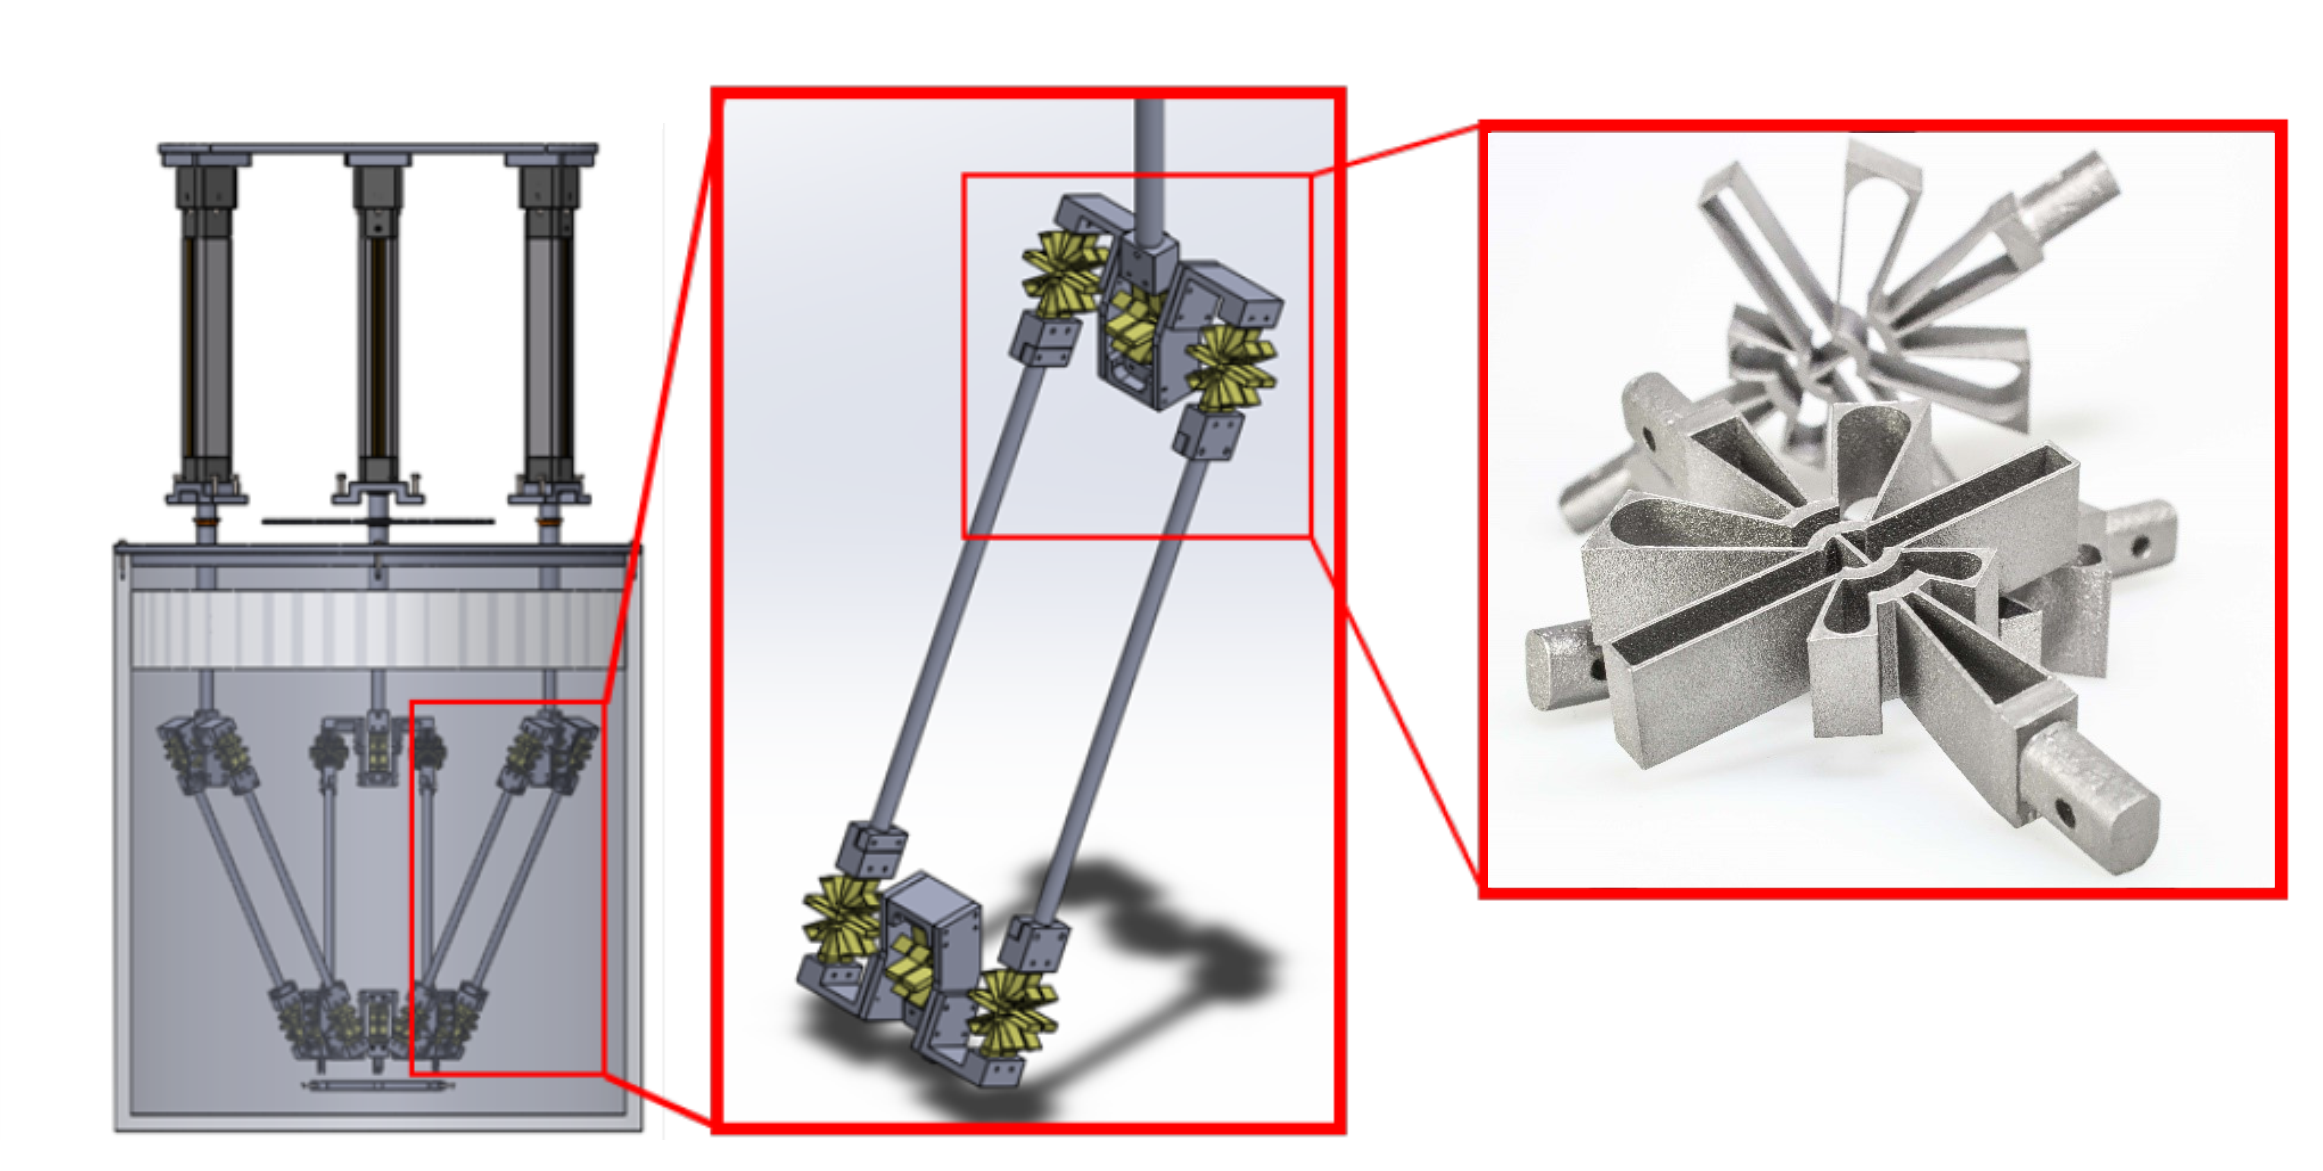
\includegraphics[width=\textwidth,height=\textheight,keepaspectratio]{figures/Demonstrator_transp.png}
    \vspace{-0.4cm} % exploit white space in image
	\caption{Left: CAD rendering of a possible parallel robot structure (from  \cite{JahnRaatz2020}), middle: detail on the leg chain, right: flexure hinge photograph}
    \vspace{-0.4cm} % bring next chapter on this page
	\label{fig:Demonstrator}
\end{figure}

\section{Engineering Approach and First Prototype}
\label{sec:engineering_synthesis}



In a first approach the selection of the parallel structure was limited to one variant:
Each kinematic leg chain consists of a vertically aligned linear drive and two passive universal joints, representing the common \emph{linear Delta robot} \cite{FrindtKreHes2010,KelaiaiaComZaa2012}, see Fig.~\ref{fig:Demonstrator}, left. 
Since both the inner and outer axes of the two universal joints are parallel to each other, a change in orientation is prevented, cf. \cite{Merlet2006,KongGos2007,Gogu2008,FrindtKreHes2010}, see Fig.~\ref{fig:Demonstrator}, middle. 

The system only has three translational degrees of freedom, required for handling the sample tubes during cryopreservation. 
In preceding works, a \textsc{Matlab} tool was developed for a dimensional synthesis of this specific structure in the confined space. 
The main goal was to determine the parameter set from the set of possible combinations of the geometric parameters, in which the required joint angle ranges of the passive, solid-state joints are minimal. 
In addition, the optimal installation angles of the passive joints were calculated, at which the deflections from the rest position are minimal. Also, a workspace analysis was carried out for the determined optimum parameter set.
A comprehensive description of the developed \textsc{Matlab} tool based on a particle swarm optimization is omitted for the sake of brevity.
The analysis showed that the optimized structure with a maximum angle range of the passive joints of only \SI{46}{\degree} experiences the least stress in the passive joints but poses the danger of singularities of the first type. 
Singularities of this type lie on the boundaries of the workspace and result, for example, from the stretching positions of individual link chains. 
It was assumed, that presetting the inclination in the universal joints to \SI{26}{\degree} would make it possible to avoid any singularities of the first type. Furthermore it was anticipated, that a larger inclination would reduce the necessary drive forces and thus result in smaller and more cost-effective drives.
Due to the nature of the kinematic chains, the working space of the developed parallel robot structure can be represented as an overlap of three cylinders, in the sectional area of which the square area to be covered is located, which contains the bearing racks and the scanner.
The minimum achievable application range of the actuator platform is, therefore a circle with the radius \SI{141.42}{\milli\metre}. 
Based on the workspace restrictions in Sec.~\ref{sec:req_robot}, the resulting bar length was calculated to \SI{334.6}{\milli\metre}. 
As an illustration, a possible configuration of the resulting parallel robot is shown in Fig.~\ref{fig:Demonstrator}. 
However, the construction shown here is only one of many possible configurations. 
With the experience gained from the reasoning of the manual design phase, the following systematic synthesis is performed in order to explore all possible solutions for the task and validate the preliminary design. 


\section{Combined Structural and Dimensional Synthesis}
\label{sec:combined_synthesis}

% number of robot structures given by number_possible_structures.m
The parallel handling robot can -- theoretically -- be built up of a vast amount of possible leg chains \cite{Gogu2008,KongGos2007}.
With a \emph{structural synthesis} similar to \cite{Gogu2008}, 51 unique leg chains consisting of revolute (R), prismatic (P) and universal (U) joints were identified for the cryogenic handling task described above.
In the following, only serial kinematic leg chains without the  parallelogram elements of Fig.~\ref{fig:Demonstrator} are selected.
In a possible design step after the synthesis, joints with parallel axes can be kinematically replaced by parallelograms \cite{FrindtKreHes2010}.
The alignment of base and platform coupling joint is not considered explicitly in textbooks on structural synthesis \cite{Gogu2008,KongGos2007}.
However, to make use of the structural synthesis in combination with the dimensional synthesis, this aspect plays a crucial part.
A general set of four possible alignments of the base coupling joint (radial, tangential, vertical or conically inclined to the base circle) and three alignments of the platform coupling joint (vertical, tangential and radial to the platform circle) are selected for evaluation.
A brute-force approach by performing the dimensional synthesis for all $51\times4\times3$ combinations without task constraints has proven to be feasible, allowing automation and avoiding symbolic calculations, e.g. of screw vectors \cite{KongGos2007}.
Not all combinations provide a feasible parallel robot with full mobility and only 328 remaining valid structures are stored in a database.
As minimizing motion in the area of thermal insulation is a hard requirement, only the vertical and conically inclined alignment of actuated prismatic base coupling joints is taken into consideration.

This leaves 33 specifiable parallel robots for the following \emph{dimensional synthesis}, where the kinematic parameters of these structures are optimized.
The 5 to 10 optimization parameters (depending on the structure) include the base and platform size and the inclination of conical base joints. 
Kinematic lengths are expressed with the Denavid-Hartenberg (DH) parameters in the notation of Khalil.
An additional offset length between the prismatic joint and the next revolute joint is added to separate joints in cold and warm areas.

The robot is modeled to be of an aluminum alloy with thin struts as hollow cylinders ($\diameter$\SI{53}{\milli\metre}, strength \SI{3}{\milli\metre}) and a thin circular platform plate (strength \SI{10}{\milli\metre}).
An additional payload of \SI{3}{\kilogram} at the platform takes the gripper into account.
The robot structure is modeled with rigid body dynamics by neglecting link elasticity \cite{SchapplerOrt2020}.
The flexure hinges, i.e. all passive joints, are assumed to have a linear joint elasticity.
The stiffness of \SI{1.4}{\newton\metre}/\SI{27.5}{\degree} is obtained using the finite element method within  \textsc{Ansys} of the joint depicted in Fig.\,\ref{fig:Demonstrator},  \cite{JahnRaatz2020}.
A reference trajectory for a pick-and-place application between the two racks as described in Sec.~\ref{sec:taskdef_requ} is simulated for 37 positions.
The inertial forces are simulated, but only play a minor part compared to forces from gravity and joint elasticities.

The \emph{overall procedure of the dimensional synthesis} of a single robot structure was extended w.r.t. the authors previous work \cite{SchapplerOrt2020} and is sketched in Fig.~\ref{fig:flowchart_optimization}.
%
% ----- Das Bild soll eigentlich direkt hier stehen. Mittlerweile ist der Text aber auf der Seite zu lang geworden.
%
\begin{figure}[tb]
\input{./figures/optimization_flowchart.pdf_tex}
\caption{Overall procedure for the dimensional synthesis of a robot}
\label{fig:flowchart_optimization}
\end{figure}
The \emph{first major step} of the fitness function for a particle is the calculation of the inverse kinematics (IK) in all configurations for the 37 reference points. 
The IK configurations (``elbow up/down'') are found by setting random initial values for the gradient-based IK algorithm and significantly change the outcome of the fitness evaluation, as constraints in this task are mostly only complied in one configuration.
The violation of a constraint immediately leads to the abortion of the current configuration with the corresponding penalty term.
After the computation of the IK, the prismatic joint offset is determined using a trust-region optimization and geometric considerations.
This slightly influences the inertial forces due to the offset's mass.
%
As a \emph{second step}, the trajectory inverse kinematics and dynamics is calculated for all valid configurations, using a general methodology \cite{Merlet2006,Gogu2008,SchapplerOrt2020}.
All constraints are again checked for the trajectory.

As the torques of the joint elasticities (considered as torsion springs) and therefore the actuator forces strongly depend on the flexure hinge rest positions, these present additional design parameters.
A choice of the rest positions in the middle of the joint range for the trajectory minimizes the spring torque, but not the actuator forces, which present the design objective.

Therefore, an additional \emph{design optimization} is performed for the rest positions of the flexure hinges as four parameters, assuming a symmetric robot.
A pretensioning of the flexure hinges within the \SI{55}{\degree} angle range was allowed, producing a partial compensation of gravity by the spring torque.
The design optimization loop is performed using a single-objective PSO minimizing the maximal actuator force.

The \emph{constraints} are checked in the order of graveness of their violation and the computational effort to determine them.
This presents a variation of the PSO ``static penalty'' approach \cite{Mezura-MontesCoe2011} (static w.r.t. iteration count), termed ``hierarchical constraints'' in this work \cite{SchapplerOrt2020}.
Examples of checked constraints in this order are
\begin{compactitem}
\item geometric plausibility (leg length matching base/platform), 
\item success of the inverse kinematics (using a gradient-based solution), 
\item range of joint angles ($<$ \SI{55}{\degree} for the flexure hinges), 
\item self-collisions (using capsules as elementary geometry and axis-aligned bounding boxes as a first check), 
\item installation space (joint positions have to be inside the cylinder of Fig.~\ref{fig:Tank}),
\item everything aforementioned for the trajectory IK,
\item condition number of the manipulator Jacobian ($<200$), 
\item actuator force in a reasonable range ($<$ \SI{100}{\newton}),
\item material stress (within a 50\% safety distance of the material's limits).
\end{compactitem}
The violation of an earlier check leads to a higher \emph{penalty term} for the fitness value, where each constraint has a reserved range of values and all constraints are continuous depending on the degree of their violation (corresponding to inequality constraints). 
Each constraint violation leads to an immediate abortion of the current iteration to reduce the computational effort. % and be able to spend the computation time on trying new particles.

By this means, the time for one fitness evaluation ranges from nearly \SI{0}{\second} (quick check for invalid geometry or failure in reference point IK) over \SI{0.5}{\second} (kinematics constraints after trajectory IK), to \SI{1.8}{\second} (full objective function without additional design optimization) and \SI{13}{\second} (including design optimization of spring rest positions with 120 evaluations of the inverse dynamics).
The computation was performed on a state-of-the-art Intel Xeon computing cluster system, using a \textsc{Matlab} implementation. % of the Leibniz University of Hannover
If all constraints are met, the maximum position error and the maximum actuator force are taken as two \emph{objective functions}, using the multi-objective PSO algorithm from \cite{CoelloPulLec2004}.
The position error is obtained by standard methods from \cite{Merlet2006} (with absolute values of the manipulator Jacobian), assuming \SI{10}{\micro\metre} encoder accuracy of the linear drives.
The physical values are normalized and saturated to a value smaller than the constraint penalties \cite{SchapplerOrt2020}.

If a constraint is violated, both fitness values are equally set to the penalty.
The feasible results and good convergence of the optimization show that the advantages of this approach (no constraint handling parameters, computationally efficient, \textsc{Matlab} implementation available \cite{CoelloPulLec2004}) prevail the disadvantages (loss of diversity in the particle swarm \cite{Mezura-MontesCoe2011}) for the optimization problem at hand.

\section{Discussion of the Results of the Synthesis}
\label{sec:results}

Using the presented framework with 9 repetitions of the dimensional synthesis, 100 generations and 100 particles each, results with qualitatively good convergence were obtained for robots 5 to 12 displayed in Fig.~\ref{fig:robot_examples1} and \ref{fig:robot_examples2}, with around 500 valid results out of the 10,000 evaluations of the fitness function.
Every optimization in this setting only takes about one to three hours (on the computing cluster), depending on the success rate and the IK convergence rate.
Robots 1 to 4 of Fig.~\ref{fig:robot_examples1} needed more evaluations, which were provided by running 50 generations with 400 particles and an initial population consisting of the best results of the previous runs.
The causing complexity of the kinematics can be deduced from the figures and the number of parameters $n$, ranging from 5 to 10.
The Pareto fronts of all repetitions are combined into one and are shown in  Fig.~\ref{fig:pareto_all}.
A position accuracy of \SI{40}{\micro\metre} was selected as a reference for the following detailed comparison in Tab.~\ref{tab:results}. 
Of the 33 different structures discussed above, 18 remain which fulfill the constraints and are regrouped for the sake of simplification (by neglecting their difference in platform coupling) to 12 remaining robots.

% Layout: Dieses Bild muss mit dem direkt hierüber liegenden Text die Seite abschließen
\begin{figure}[b!]
\vspace{-0.7cm} % zum Zusammenhalten des ersten Teils von Kapitel 5
\centering
\input{./figures/robots2.pdf_tex}
\vspace{-0.7cm}
\caption{Visualization of selected robot kinematics from Tab.~\ref{tab:results} with markers from Fig.~\ref{fig:pareto_all}. Leg chains are printed in different colors and the circle marks the tank's upper edge.}
\label{fig:robot_examples1}
\end{figure} 

\begin{figure}[p]
%\vspace{-0.3cm} % Keep everything on page. Not allowed on top
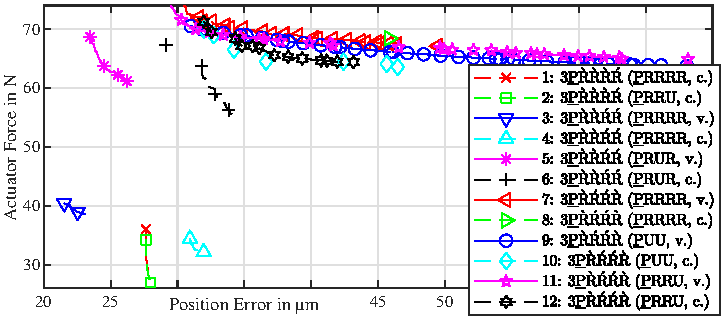
\includegraphics{pareto_all.pdf}
\vspace{-0.8cm} % Keep everything on page.
\caption{Pareto fronts for all robot structures. The parallel robot notation is taken from \cite{Merlet2006} and the kinematic chain notation is taken from \cite{KongGos2007}, where all \`R and \'R are parallel to each other, respectively. Base alignment noted with ``v'' (vertical) and ``c'' (conical).}
\label{fig:pareto_all}
\end{figure}
%
% Zum Eintragen der Marker-Symbole in den Text. Matlab erzeugt immer einen geringen weißen Rand darum herum. Am einfachsten hier direkt zuschneiden.
% https://tex.stackexchange.com/a/17101
\newcommand{\vcenteredinclude}[1]{\begingroup
	\setbox0=\hbox{\includegraphics[trim=0.3mm 0.3mm 0.3mm 0.3mm, clip, height=3.5mm]{#1}}%
	\parbox{\wd0}{\box0}\endgroup}
%
\begin{table}[p]
\centering
\caption{Summary of one typical particle for each robot from the Pareto front. Abbreviations: ``cond.'' (condition number of Jacobian), range (of passive joint angles), mass (articulated, legs and platform without payload), $n$ (number of optimization variables), $r_\mathrm{B}$ (base radius), $\varphi_\mathrm{B}$ (prismatic joint inclination), $r_\mathrm{P}$ (platform radius), $q_{1\mathrm{off}}$ (prismatic joint offset), $a_i$,$d_i$ (DH parameters). Row ``Eng.'': engineering solution from Fig.~\ref{fig:Demonstrator}.}
\vspace{-0.5cm} % Keep everything on page
\begin{tabular}[t]{|c c|r|r|r|r|r|r|r|r|r|r|r|r|r|r|r|}
\hline
& & \multicolumn{5}{c|}{\textbf{performance}} & \multicolumn{10}{c|}{\textbf{kinematic parameters}} \\
\hline
& & \multicolumn{1}{r|}{err.} & \multicolumn{1}{r|}{force} & \multicolumn{1}{r|}{cond.} & \multicolumn{1}{c|}{range} &  \multicolumn{1}{c|}{mass} & \multicolumn{1}{c|}{$n$} &
\multicolumn{1}{c|}{$r_\mathrm{B}$} & \multicolumn{1}{c|}{$\varphi_\mathrm{B}$} & \multicolumn{1}{c|}{$r_\mathrm{P}$} & \multicolumn{1}{c|}{$q_{1\mathrm{off}}$} & \multicolumn{1}{c|}{$a_3$} & \multicolumn{1}{c|}{$d_3$} & \multicolumn{1}{c|}{$a_4$} & \multicolumn{1}{c|}{$d_4$} & \multicolumn{1}{c|}{$a_5$} \\
& & \multicolumn{1}{c|}{\SI{}{\micro\metre}}  & \multicolumn{1}{c|}{N} & \multicolumn{1}{c|}{} & \multicolumn{1}{c|}{deg} & \multicolumn{1}{c|}{kg} & & \multicolumn{1}{c|}{mm} & \multicolumn{1}{c|}{mm} & \multicolumn{1}{c|}{deg} & \multicolumn{1}{c|}{mm} & \multicolumn{1}{c|}{mm} & \multicolumn{1}{c|}{mm} & \multicolumn{1}{c|}{mm} & \multicolumn{1}{c|}{mm} & \multicolumn{1}{c|}{mm} \\
\hline
% table data generated by results_tables_latex.m
1 & \vcenteredinclude{tables/group1_marker.pdf} & 28 & 28 & 1.2 & 51.0 & 4.3 & 10 & $374$ & $59$ & $81$ & $208$ & $263$ & $135$ & $332$ & $144$ & $24$ \\ % cryopkm_20210122_newcoll_nobase_ga_ps11_rep1/Rob1_P3PRRRR3G4P2A1 (Pareto-Index 16)
2 & \vcenteredinclude{tables/group2_marker.pdf} & 28 & 27 & 1.1 & 49.3 & 4.2 & 9 & $359$ & $57$ & $83$ & $200$ & $271$ & $164$ & $309$ & $127$ & \multicolumn{1}{c|}{---} \\ % cryopkm_20210126_refine3_ga_ps11_rep2/Rob2_P3PRRRR3V1G4P2A1 (Pareto-Index 146)
\hline
3 & \vcenteredinclude{tables/group3_marker.pdf} & 23 & 39 & 5.3 & 53.7 & 6.1 & 8 & $223$ & $0$ & $80$ & $408$ & $330$ & $106$ & $151$ & $91$ & $390$ \\ % cryopkm_20210126_refine3_ga_ps11_rep2/Rob4_P3PRRRR6G1P3A1 (Pareto-Index 97)
4 & \vcenteredinclude{tables/group4_marker.pdf} & 32 & 32 & 3.5 & 46.8 & 5.1 & 9 & $297$ & $50$ & $80$ & $212$ & $314$ & $316$ & $151$ & $118$ & $233$ \\ % cryopkm_20210126_refine3_ga_ps11_rep2/Rob5_P3PRRRR6G4P2A1 (Pareto-Index 46)
5 & \vcenteredinclude{tables/group5_marker.pdf} & 26 & 61 & 2.5 & 46.7 & 4.2 & 6 & $206$ & $0$ & $80$ & $235$ & $282$ & $150$ & \multicolumn{1}{c|}{---} & \multicolumn{1}{c|}{---} & $307$ \\ % cryopkm_20210122_newcoll_nobasexx_ps11_rep3/Rob6_P3PRRRR6V1G1P3A1 (Pareto-Index 25)
6 & \vcenteredinclude{tables/group6_marker.pdf} & 34 & 56 & 2.5 & 53.0 & 3.7 & 7 & $252$ & $30$ & $80$ & $164$ & $275$ & $229$ & \multicolumn{1}{c|}{---} & \multicolumn{1}{c|}{---} & $222$ \\ % cryopkm_20210122_newcoll_nobase_ga_ps11_rep2/Rob7_P3PRRRR6V1G4P2A1 (Pareto-Index 48)
\hline
7 & \vcenteredinclude{tables/group7_marker.pdf} & 40 & 69 & 3.8 & 40.8 & 3.6 & 8 & $225$ & $0$ & $80$ & $158$ & $165$ & $52$ & $321$ & $143$ & $34$ \\ % cryopkm_20210122_newcoll_nobase_ga_ps11_rep2/Rob10_P3PRRRR8G1P3A1 (Pareto-Index 19)
8 & \vcenteredinclude{tables/group8_marker.pdf} & 44 & 81 & 3.8 & 40.3 & 3.8 & 9 & $177$ & $174$ & $81$ & $367$ & $109$ & $28$ & $258$ & $47$ & $20$ \\ % cryopkm_20210122_newcoll_nobasexx_ps11_rep2/Rob11_P3PRRRR8G4P2A1 (Pareto-Index 1)
9 & \vcenteredinclude{tables/group9_marker.pdf} & 40 & 67 & 3.4 & 36.9 & 3.6 & 5 & $225$ & $0$ & $80$ & $369$ & \multicolumn{1}{c|}{---} & \multicolumn{1}{c|}{---} & $347$ & $41$ & \multicolumn{1}{c|}{---} \\ % cryopkm_20210126_refine3_ps11_rep2/Rob13_P3PRRRR8V1G1P2A1 (Pareto-Index 22)
10 & \vcenteredinclude{tables/group10_marker.pdf} & 42 & 64 & 3.9 & 33.5 & 3.6 & 6 & $191$ & $172$ & $80$ & $306$ & \multicolumn{1}{c|}{---} & \multicolumn{1}{c|}{---} & $399$ & $104$ & \multicolumn{1}{c|}{---} \\ % cryopkm_20210122_newcoll_nobasexx_ps11_rep3/Rob14_P3PRRRR8V1G4P2A1 (Pareto-Index 3)
11 & \vcenteredinclude{tables/group11_marker.pdf} & 40 & 68 & 3.8 & 40.5 & 3.6 & 7 & $225$ & $0$ & $80$ & $153$ & $204$ & $97$ & $323$ & $94$ & \multicolumn{1}{c|}{---} \\ % cryopkm_20210122_newcoll_nobase_ga_ps11_rep1/Rob16_P3PRRRR8V2G1P3A1 (Pareto-Index 34)
12 & \vcenteredinclude{tables/group12_marker.pdf} & 40 & 65 & 3.5 & 34.4 & 3.7 & 8 & $207$ & $174$ & $80$ & $327$ & $22$ & $38$ & $374$ & $69$ & \multicolumn{1}{c|}{---} \\ % cryopkm_20210122_newcoll_nobase_ga_ps11_rep1/Rob17_P3PRRRR8V2G4P2A1 (Pareto-Index 11)
\multicolumn{2}{|c|}{Eng.} & 37 & 67 & 3.1 & 39.3 & 3.6 & 6 & $230$ & $0$ & $80$ & $395$ & \multicolumn{1}{c|}{---} & \multicolumn{1}{c|}{---} & $335$ & $0$ & \multicolumn{1}{c|}{---} \\ % Engineering Solution; see eval_existing_design.m

\hline
\end{tabular}
\label{tab:results}
\end{table}
%
\begin{figure}[p]
\vspace{-0.2cm} % Keep everything on page
\centering
\input{./figures/robots3.pdf_tex}
\caption{Second half of the robot kinematics visualizations from Tab.~\ref{tab:results}.}
\label{fig:robot_examples2}
\end{figure} 

The structures 1 to 4 are clearly dominant over all others due to their actuation force lower than \SI{40}{\newton}. 
However, the kinematic structure of numbers 3 and 4, visible in Fig.~\ref{fig:robot_examples1}, is significantly more complicated than the engineering solution (structure 9 in  Fig.~\ref{fig:robot_examples2}), making their realization less likely.
Structures 1 and 2 have moderate complexity and are even able to reach full isotropy ($\mathrm{cond}(\bm{J})=1$ in the whole workspace) for some particles on the Pareto front, which generally is very favorable \cite{Gogu2008}.
A detailed analysis shows that a low actuator force in general is mainly enabled by a compensation of the effects of gravity and joint elasticity, together with a good force transmission from actuators to platform.
From other runs of the optimization it is known that passive joint angle ranges of only \SI{22}{\degree} are possible for some structures, but the optimal results are over \SI{40}{\degree}.
Therefore minimizing the angle range or the elastic joint torque does not directly benefit this objective, supporting the results from Sec.~\ref{sec:engineering_synthesis}

The 3\underline{P}RUR-structures (numbers 5 and 6) present the second best alternative, as an actuator force of \SI{56}{\newton} can be achieved with a conical alignment of the prismatic joints.
The engineering solution of Sec.~\ref{sec:engineering_synthesis} corresponds to the 3\underline{P}UU-kinematics (number 9), which has a similar performance as structures number 7 to 12.
The engineering solution is evaluated in the last row of the table and also lies on the Pareto front, validating the different tools.
All these structures (number 7 to 12) have a similar parallel and vertical alignment of joint axes, noted by \`R\'R\'R\`R.
The main difference between numbers 7/8, 9/10 and 11/12 is the replacement of \`R\'R-pairs of revolute joints by universal joints, which sets the intermediate DH parameters to zero, but does not change the kinematic structure.
For these structures a conical joint alignment is not sufficiently beneficial.

\section{Summary and Outlook}
\label{sec:summary}

Enhancing the assumptions in the combined structural and dimensional robot synthesis with knowledge from the engineering approach allows to vastly reduce the complexity of the optimization problem, without limiting the combined synthesis in the highly constrained cryogenic handling task.
The comparison already proves the feasibility of the chosen design relative to other possible structures.
The theoretical improvement of a design change is quantified to reduce the already low actuator force about 60\%.
This would require using two single revolute joints instead of one universal joint and may reduce the structural stiffness.
Further investigations on replacing consecutive parallel joints by parallelogram subchains have to be performed before considering the design change.
The findings on compensating gravity with elastic joint moments may be used in a pretensioning of the flexure hinges and in the control of the robot.


\section*{Acknowledgements}
\vspace{-0.2em}
The authors acknowledge the support by the Deutsche Forschungsgemeinschaft (DFG) under project numbers 341489206 (combined synthesis) and 349906175 (cryogenic handling).
%
\textsc{Matlab} Code to reproduce the results is available at GitHub under
\url{https://github.com/SchapplM/robsynth-paper_mhi2021}.
\vspace{-0.2em}

%
% ---- Bibliography ----
%
% BIBLIOGRAPHY
\bibliographystyle{spmpsci_unsrt}
\bibliography{references}
\end{document}
